\documentclass[oneside, class=book, crop=false, 12pt]{standalone}

\usepackage{../dissertationstyle}

\bibliography{../personal}

\begin{document}


\ifstandalone
  \setcounter{chapter}{0}
  \chapter{Introduction}
\fi
\resetfigpath{introduction}

This chapter explains the motivation for this project, provides an overview of the project and how it works, and discusses previous related work in this area.

\section{Motivation}

Individuals have many characteristics that can be used to identify them, ranging from immutable characteristics of a person like biometrics, to qualities of an action they perform, such as their handwriting. This project explores the use of another characteristic that can be used to identify a person: how they play a particular piece on the piano. 

Suppose a famous pianist dies, and a number of demo recordings of their pieces are found that could be worth a lot of money. With the pianist dead, it is hard to determine the authenticity of these recordings, and the ability to identify the performer of these recordings would be very useful in order to properly assess the value of the recordings. Another example use case might be in court: if a pianist wants to provide an alibi of some audio recording taken at the time they are accused of committing a crime, then such a tool that is able to verify the integrity of this alibi by providing a quantitative statement of how similar the audio recording is to their actual playing would be very useful to provide to a jury, especially if the jury has no musical experience.

\section{Project Mechanism and Overview}

In order to pull useful information out of an audio recording related to a pianist's performance, we need to process the signal in some meaningful way to gather musical information from it. For example, the discrete-time Fourier transform (DTFT) is used to transform a discrete-time audio signal into its frequency data. This technique is invaluable and has a myriad of uses, for example being able to get data about what notes are being played at a given time, or to attempt to quantify the timbre of a particular sound.




The system created in this project works as follows: given performances of the same piece by different pianists, we compute a number of metrics for each performance and store them. To try and determine the performer of a performance with an unknown performer, we compute the same metrics on this performance, and then compute similarities between the metrics of this performance and the metrics of the other performances, and choose the performer for which we get the highest aggregate similarity.

In total, the project implements five metrics:

\begin{itemize}
  \item
    Tempo variation over time:

    This metric tracks how the tempo, how fast or slow the piece is being played, changes over the performance of a piece. Figure \ref{figure:tempoplot} visualises this metric by plotting the distance of note onsets from the expected note onset if the piece were played at a fixed tempo.

\begin{minipage}{\textwidth}
  \centering
  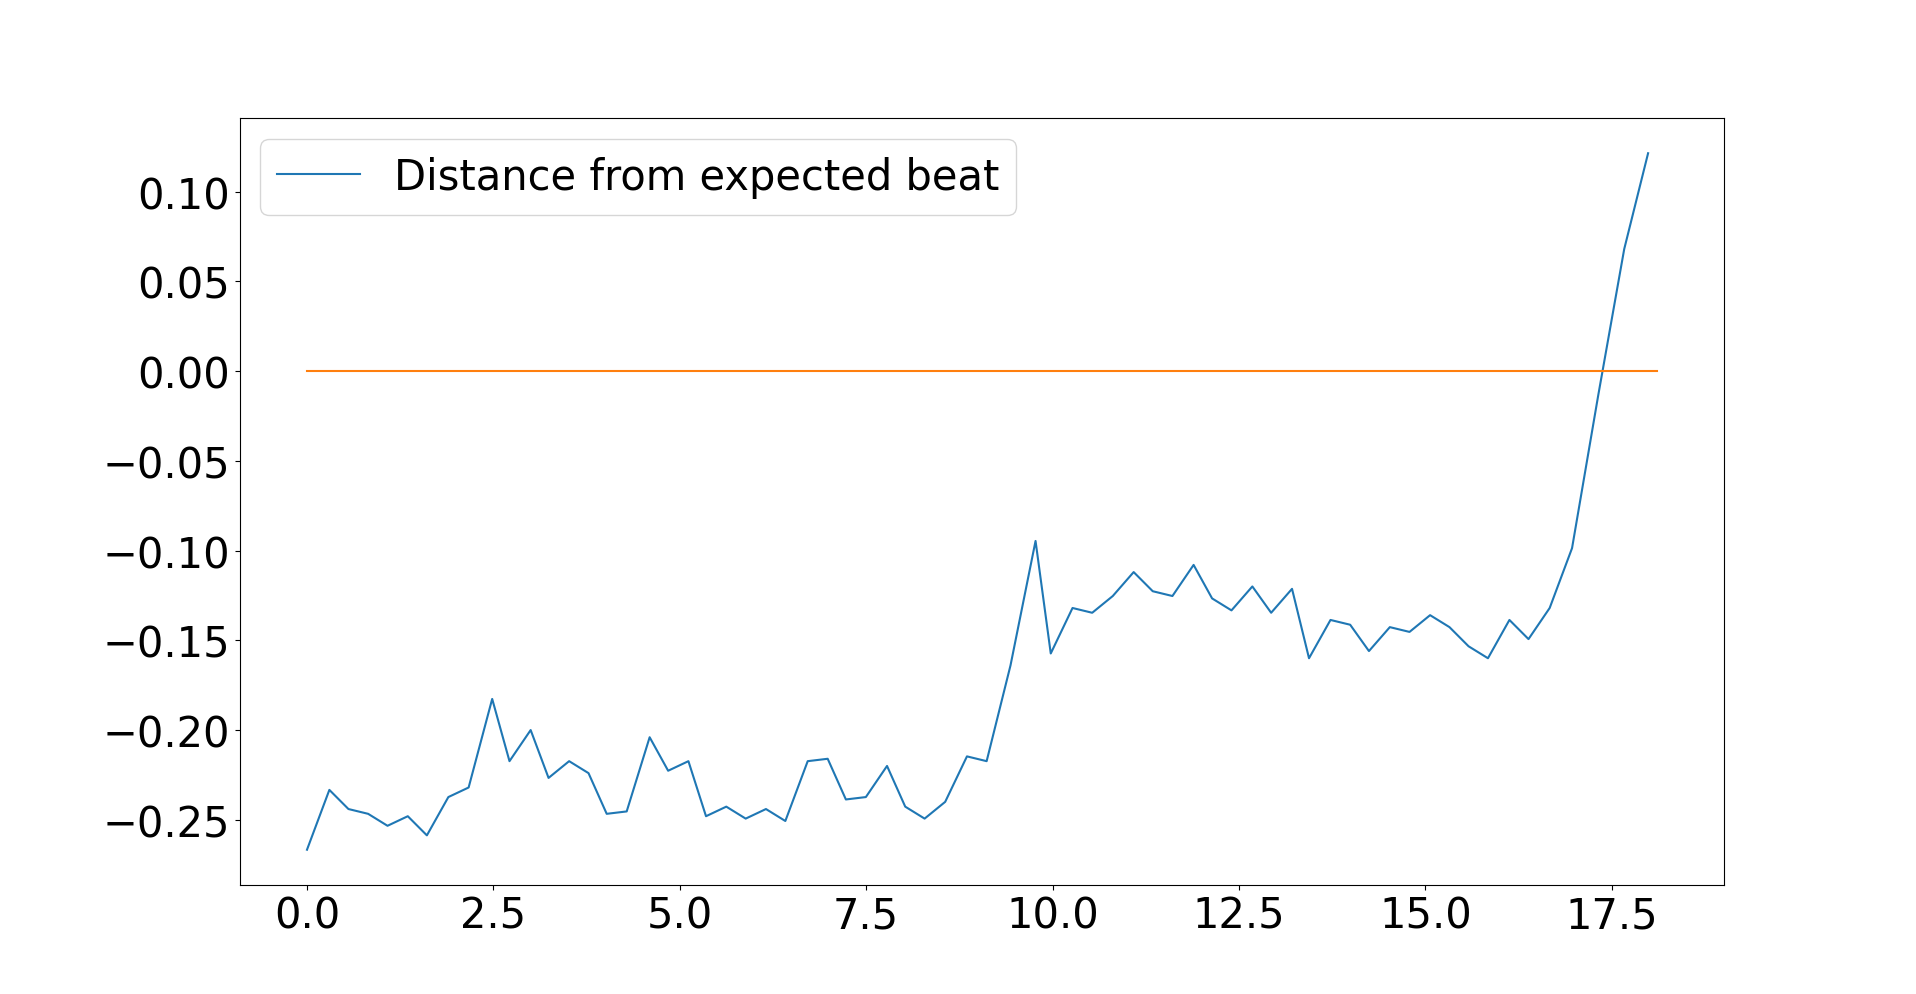
\includegraphics[scale=0.3]{tempoplot}
  \captionof{figure}{Tempo variation compared to a steady tempo}\label{figure:tempoplot}
\end{minipage}

  \item
    Dynamics over time:

    This metric tracks how the tempo, the loudness of a performance, changes over the performance of a piece. Figure \ref{figure:dynamicsplot} visualises this metric by plotting this metric against the audio signal.

\begin{minipage}{\textwidth}
  \centering
  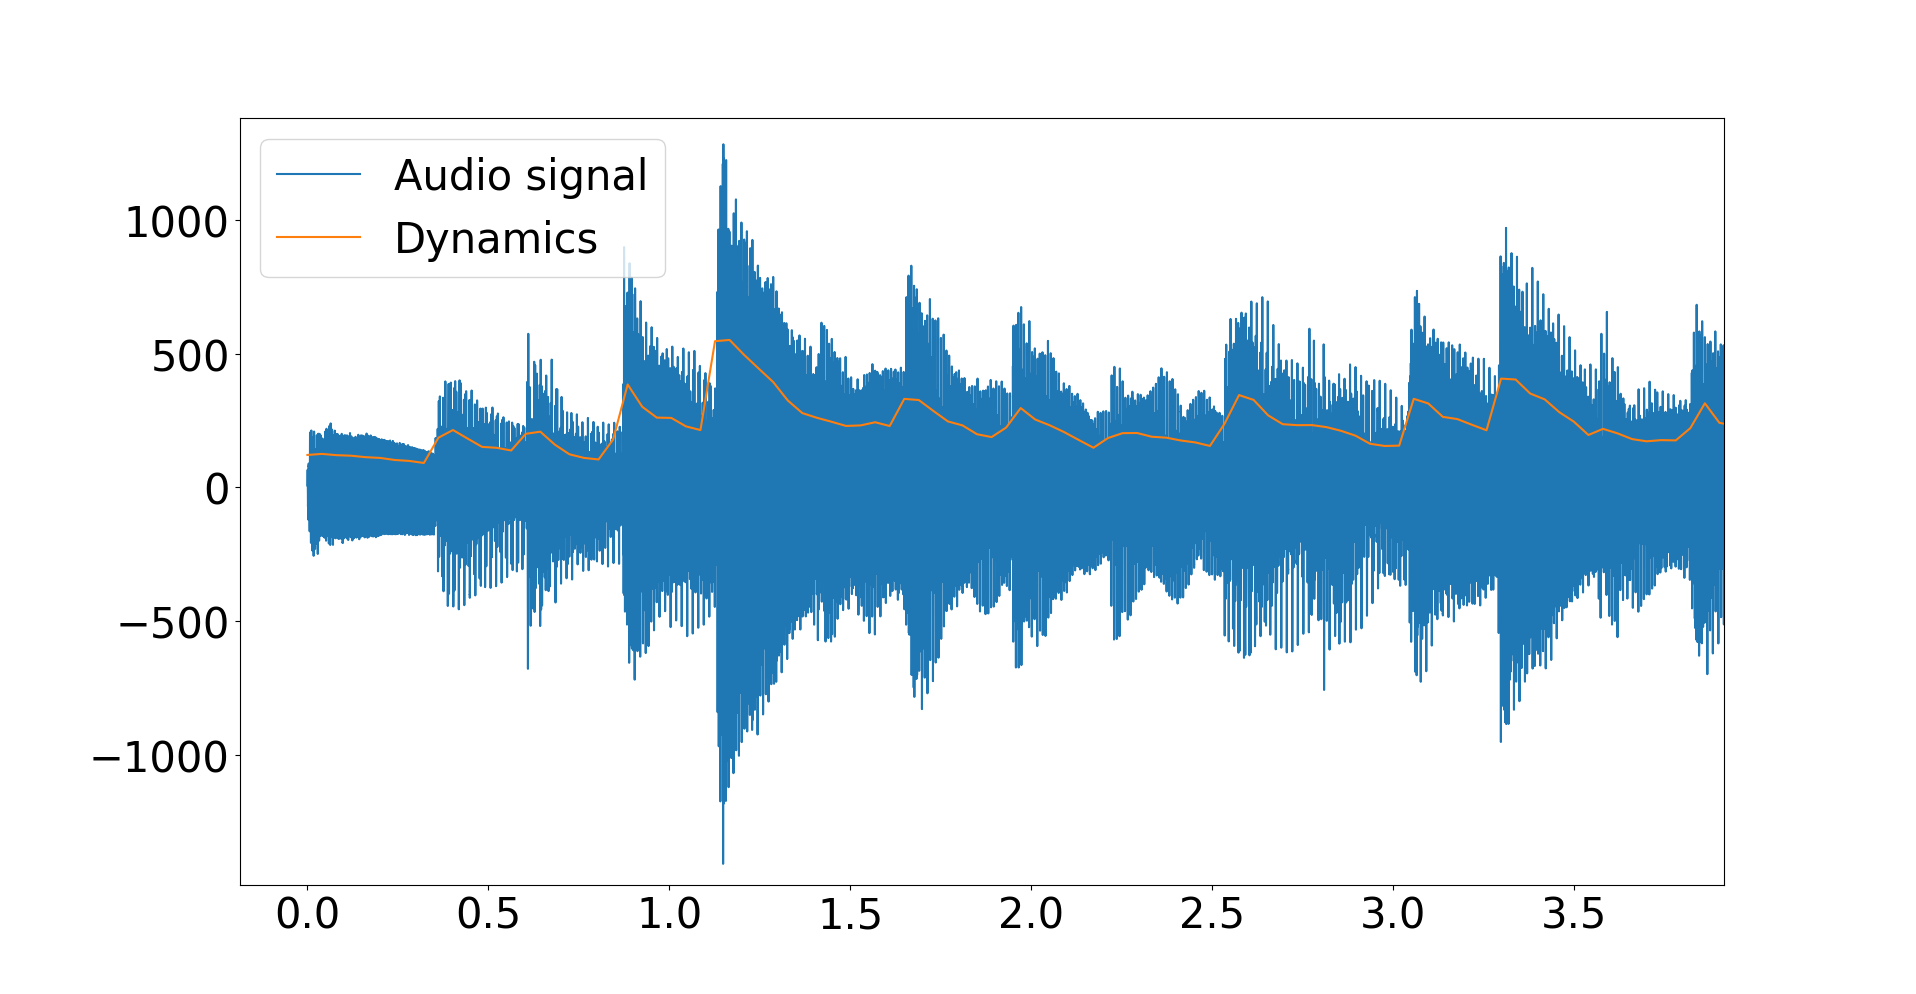
\includegraphics[scale=0.3]{dynamicsplot}
  \captionof{figure}{Dynamics of a performance}\label{figure:dynamicsplot}
\end{minipage}


  \item
    Chroma vector extraction:

    This metric tries to track what notes are being played at a given time, by observing the power in frequency bands corresponding to each note.

  \item
    Note offsets:

    This metric tries to track micro-timing differences in the performance of a piece by comparing the actual note onsets to the expected note onset. Figure \ref{figure:offsetsplot} visualises this by plotting expected note onsets and actual note onsets.

\begin{minipage}{\textwidth}
  \centering
  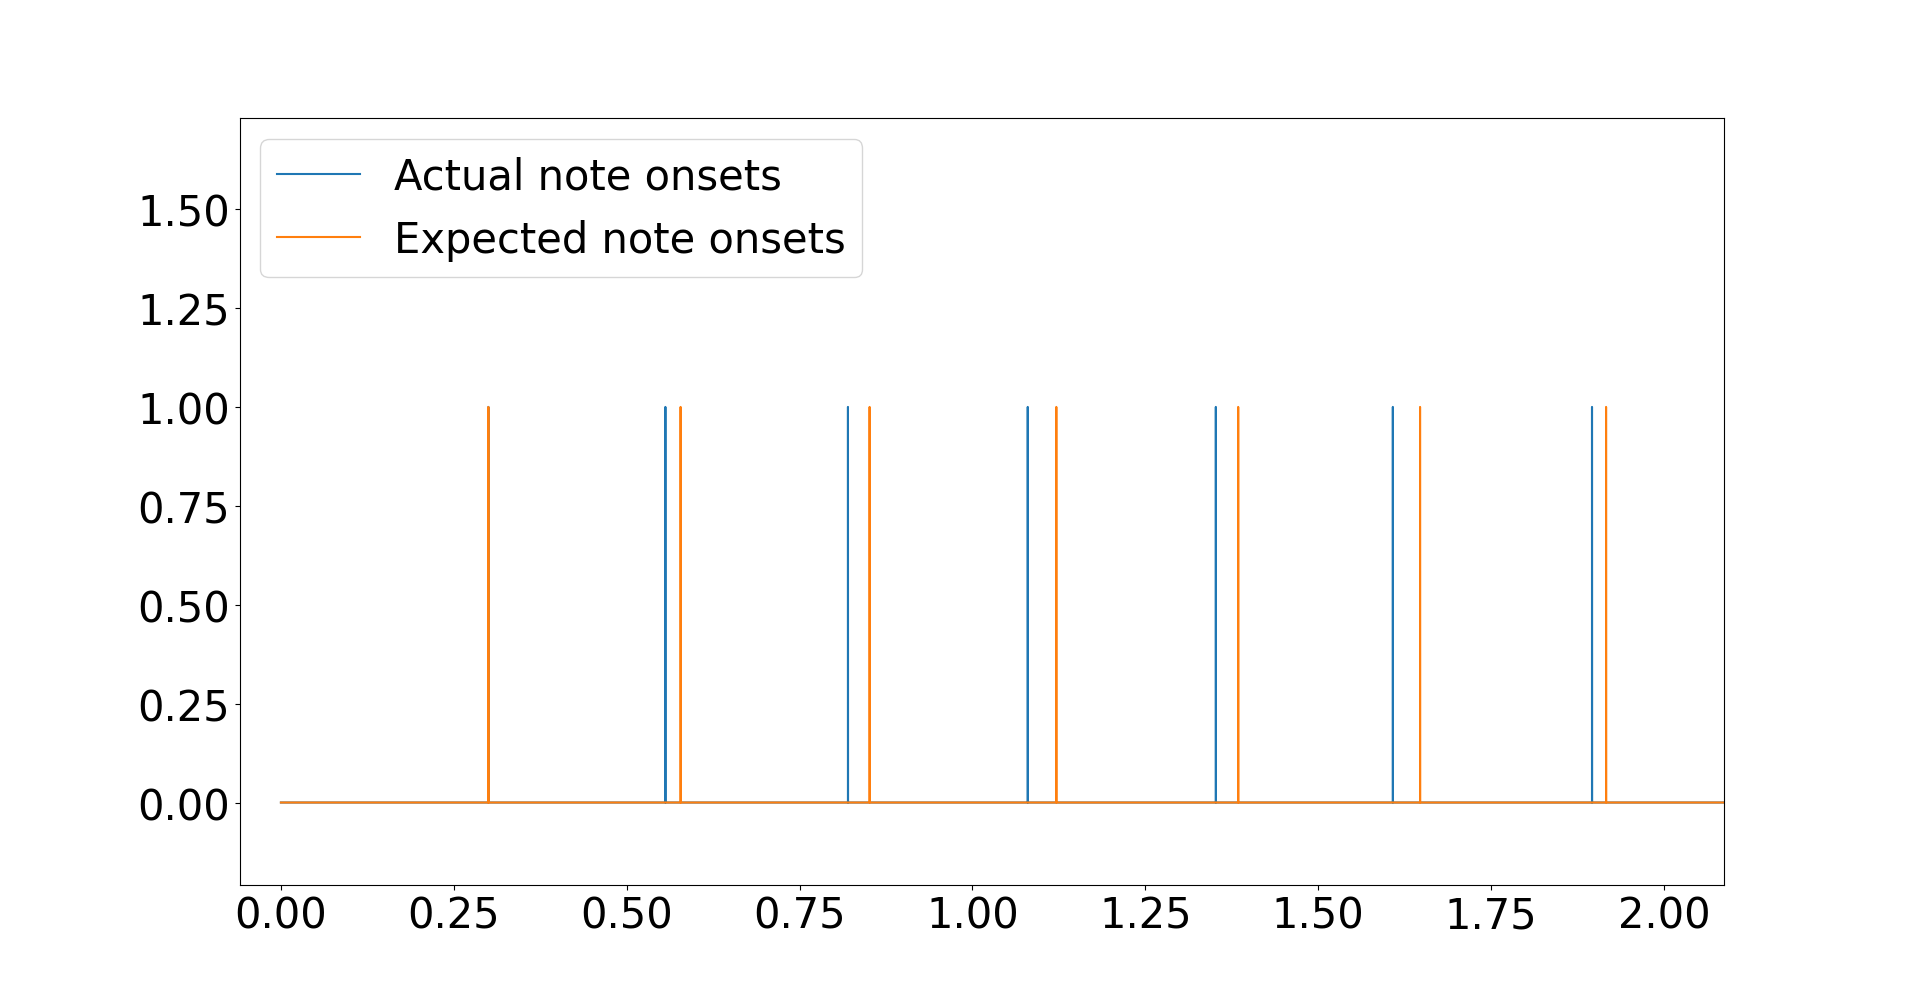
\includegraphics[scale=0.3]{offsetplot}
  \captionof{figure}{Actual note onsets compared to expected note onsets}\label{figure:offsetsplot}
\end{minipage}



  \item
    Timbre extraction:

    This metric tries to quantify the timbre of the piece over time. It should be noted that this is a known hard problem in the field of music information retrieval, meaning that grasping a semantic meaning of this metric is quite difficulte
\end{itemize}





An explanation of how we compute each of these metrics, and what form they take is given in Chapter \ref{chapter:implementation}

The project explores which of these metrics are most useful, and quantifies the usefulness of each metric, and looks at how the metrics perform under different conditions (e.g. addition of white noise).


\section{Related work}

There is some relevant work already done that is adjacent to this topic, for example there is a paper that investigates how individual a pianist's performance is, exploring many different metrics \cite{bernays14}, but this paper uses a symbolic representation of the performances with MIDI, as opposed to audio of the performance itself.

There is no similar work that operates on audio signals as far as I am aware, but there is some work that uses raw audio signals of a sung password using the timbre of the voice as biometric authentication \cite{prakash16}, which whilst not the same as the work in this project, is relevant.

Furthermore, there is plenty of research on beat tracking, in particular we use the techniques by Ellis \cite{ellis07}, which is a vital component of our project.


\ifstandalone
  \printbibliography[heading=subbibliography]
\fi
    
\end{document}
